\chapter{تجارب جهانی و کشورهای پیشرو}
\label{chap:global}
%=====================================================================

\section{چین: کریدور ملی پکن-شانگهای}

چین بزرگ‌ترین و بلندترین شبکهٔ \lr{QKD} مبتنی بر فیبر جهان را در اختیار دارد. کریدور پکن-شانگهای با طول بیش از $2000$ کیلومتر، شهرهای پکن، جینان، هفی و شانگهای را با استفاده از $32$ گرهٔ مورد اعتماد به‌هم متصل می‌کند و از فیبر تاریک اختصاصی در طول‌موج $1550$ نانومتر با پروتکل‌های آماده‌سازی-و-اندازه‌گیری بهره می‌برد \Cite{jrc2019qkd}. این کریدور به شبکه‌های کلان‌شهری پکن، شانگهای، هفی ($46$ گره) و جینان ($56$ گره) نیز متصل است \Cite{jrc2019qkd}.

علاوه‌بر شبکهٔ زمینی، چین از طریق ماهوارهٔ \lr{Micius} (پرتاب‌شده در سال $2016$ توسط آکادمی علوم چین) نخستین پیوند \lr{QKD} ماهواره‌ای-زمینی جهان را برقرار کرده است. این ماهواره با اتصال ایستگاه‌های زمینی \lr{Xinglong} و \lr{Nanshan} در فاصلهٔ $2600$ کیلومتری از یکدیگر \Cite{npl2020progress}، و همچنین با ارتباط بین‌قاره‌ای پکن-وین در فاصلهٔ بیش از $1200$ کیلومتر \Cite{arxiv1809largescale}، کارایی سامانه‌های مبتنی بر فیبر را به‌شدت ارتقا داده است. در این معماری، ماهواره به‌عنوان یک \textbf{گرهٔ مورد اعتماد پرنده} عمل می‌کند: هر ایستگاه زمینی به‌طور مستقل با ماهواره کلید تبادل می‌کند و ماهواره کلید مشترک نهایی را میان دو ایستگاه توزیع می‌کند (شکل \ref{fig:satellite}). با ادغام این پیوند ماهواره‌ای با کریدور زمینی پکن-شانگهای، چین شبکه‌ای با پوشش کلی بیش از $4600$ کیلومتر و حدود $150$ کاربر ایجاد کرده که نخستین نمونهٔ شبکهٔ \lr{QKD} در مقیاس بین‌قاره‌ای محسوب می‌شود \Cite{csis2026china}. در ادامهٔ این روند، ماهوارهٔ سبک‌تر \lr{Jinan-1} (با وزن تنها $23$ کیلوگرم در برابر $250$ کیلوگرم ماهوارهٔ \lr{Micius}) در سال $2022$ توسط دانشگاه علوم و فناوری چین \lr{(USTC)} و شرکت \lr{QuantumCTek} به مدار فرستاده شد که امکان استقرار سریع‌تر و کم‌هزینه‌تر ایستگاه‌های زمینی قابل‌حمل را نشان داد \Cite{tqi2026pqccompanies}.

\begin{figure}[htbp]
\centering
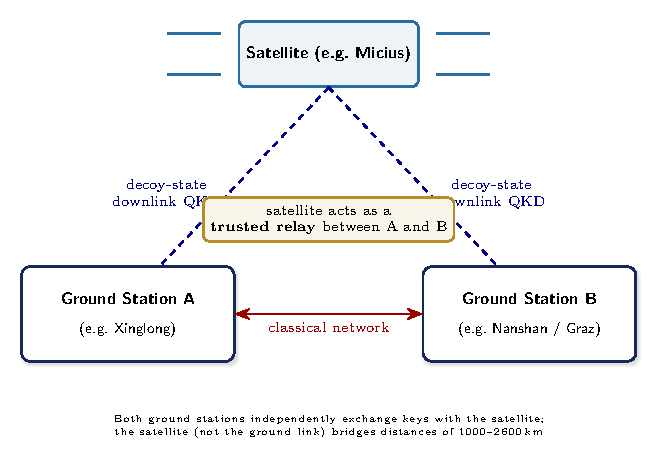
\includegraphics[width=0.85\linewidth]{figs/fig_satellite_qkd.pdf}
% TODO: لوگو، در صورت تمایل، لوگوی آکادمی علوم چین یا USTC را اینجا اضافه کنید
\caption{معماری کلی \lr{QKD} ماهواره‌ای با ماهواره در نقش گرهٔ مورد اعتماد (الگوبرداری‌شده از تجربهٔ ماهوارهٔ \lr{Micius}) \Cite{arxiv2605satreview,arxiv1809largescale}}
\label{fig:satellite}
\end{figure}

رویکرد چین، سرمایه‌گذاری دولت‌محور و یکپارچه در شبکه‌های دولتی، مالی و ارتباطات حیاتی، هم‌زمان با نقش‌آفرینی فعال در نهادهای استانداردسازی بین‌المللی نظیر کمیتهٔ مشترک \lr{IEC/ISO} با عنوان \lr{JTC 3} است \Cite{iiss2026governance}. شرکت \lr{QuantumCTek}، که توسط دانشمندان برجستهٔ \lr{USTC} از جمله «پدر کوانتوم چین»، پن جیان‌وی\LTRfootnote{Pan Jianwei (also romanized as Jian-Wei Pan)}، تأسیس شده، به‌عنوان یکی از اصلی‌ترین تأمین‌کنندگان تجهیزات این کریدور ملی شناخته می‌شود \Cite{itif2024china}.

\section{اروپا: پروژهٔ \lr{EuroQCI} و نمونهٔ سوئد}

اتحادیهٔ اروپا از طریق برنامهٔ زیرساخت ارتباطات کوانتومی اروپا \lr{(EuroQCI)} در حال ساخت بخش‌های ملی شبکهٔ کوانتومی است. یک نمونهٔ برجستهٔ اخیر، پیوند $303$ کیلومتری در سوئد است که با ترکیب آشکارسازهای نانوسیم ابررسانا \lr{(SNSPD)} و سوئیچینگ فیبر چندهسته‌ای فعال، یک گرهٔ مورد اعتماد تنها میان لینشوپینگ و استکهلم را پوشش می‌دهد \Cite{arxiv2606sweden,techtimes2026sweden}. این معماری تک‌گره‌ای، در مقایسه با ده‌ها گرهٔ مورد نیاز در طرح‌های قدیمی‌تر، نشان‌دهندهٔ کاهش چشمگیر سطح حملهٔ قابل‌بهره‌برداری \lr{(Attack Surface)} است، هرچند به قیمت هزینهٔ بالای آشکارسازهای ابررسانا (در حدود $100000$ یورو برای هر سامانهٔ \lr{SNSPD} به‌همراه نیاز به زیرساخت سرمایشی) تمام می‌شود \Cite{techtimes2026sweden}.

\section{سنگاپور، ژاپن و کرهٔ جنوبی}

سنگاپور در حال ساخت یک مش \lr{QKD} در سطح کل کشور، شبکهٔ \lr{National Quantum-Safe Network Plus (NQSN+)}، برای حفاظت از جایگاه خود به‌عنوان مرکز مالی آسیا است \Cite{marketintelo2026}. ژاپن و کرهٔ جنوبی نیز نقشهٔ راه ملی \lr{QKD} خود را هم‌زمان با برنامه‌های زیرساخت مخابراتی نسل ششم \lr{(6G)} پیش می‌برند؛ در کرهٔ جنوبی، یک شبکهٔ ترکیبی میان سئول و بوسان به طول تقریبی $490$ کیلومتر در دست ساخت است \Cite{npl2020progress}.

\section{ایالات متحده}

ایالات متحده، در کنار سرمایه‌گذاری بانک‌های خصوصی نظیر \lr{JPMorgan Chase} (بخش \ref{sec:bankexperience})، از طریق آزمایشگاه‌های ملی و برنامه‌های \lr{NIST}، نصب شبکه‌های آزمایشی \lr{QKD} خود را آغاز کرده است \Cite{npjqi2016}. با این حال، رویکرد رسمی نهادهای امنیتی آمریکا (\lr{NSA}) عمدتاً بر \lr{PQC} به‌عنوان مسیر اصلی مهاجرت سامانه‌های امنیت ملی متمرکز است، در حالی که \lr{QKD} را بیشتر برای کاربردهای خاص و مکمل توصیه می‌کنند \Cite{techtimes2026sweden}.

\section{وضعیت و ظرفیت داخلی جمهوری اسلامی ایران}
\label{sec:iran}

بررسی منابع علمی و خبری در زمان تدوین این سند (مرداد \lr{1405}) نشان می‌دهد که ایران نیز، هرچند در مقیاسی کوچک‌تر از بازیگران فصل حاضر، فعالیت رسمی و آکادمیک در این حوزه را آغاز کرده است:

\begin{itemize}
\item \textbf{شبکهٔ ملی کوانتومی:} به گزارش خبرگزاری \lr{Tehran Times}، وزارت ارتباطات و فناوری اطلاعات اعلام کرده که نخستین شبکهٔ ملی کوانتومی کشور با هدف بهره‌برداری تا اسفند \lr{1404} (حدود مارس \lr{2026}) در دست طراحی و اجراست؛ این پروژه با حمایت وزارت ارتباطات، سازمان انرژی اتمی و شرکت‌های دانش‌بنیان از طریق مطالعهٔ تطبیقی برنامه‌های کشورهای پیشرو آغاز شده است \Cite{tehrantimes2025network}. بر اساس همین گزارش، رتبهٔ ایران در تولید علم حوزهٔ فناوری‌های کوانتومی (بر مبنای پایگاه \lr{Web of Science}) از رتبهٔ $23$ در سال $2014$ به رتبهٔ $16$ در سال $2023$ ارتقا یافته است.
\item \textbf{آزمایشگاه ارتباطات کوانتومی:} در مهر \lr{1404} (اکتبر \lr{2025})، تأسیس نخستین «آزمایشگاه ارتباطات کوانتومی و ساعت اتمی» کشور اعلام شد؛ $55\%$ از تأمین مالی این آزمایشگاه بر عهدهٔ معاونت علمی، فناوری و اقتصاد دانش‌بنیان ریاست‌جمهوری و بخش دیگر آن با همکاری پژوهشگاه ارتباطات و فناوری اطلاعات خواهد بود \Cite{tqi2025iranlab}.
\item \textbf{پیشینهٔ آزمایش‌های اولیه:} گزارش‌های قدیمی‌تر صنعتی نشان می‌دهند که سازمان انرژی اتمی ایران پیش‌تر (حدود سال \lr{1399}) از انجام «فاز سوم آزمون‌های توزیع کلید کوانتومی» در کشور خبر داده بود \Cite{iqt2021iranqkd}، شاهدی بر آنکه این حوزه از چند سال پیش در دستور کار پژوهشی کشور قرار داشته است.
\item \textbf{پژوهش دانشگاهی:} گروه پژوهشی «آزمایشگاه فوتونیک» دانشکدهٔ مهندسی برق دانشگاه صنعتی امیرکبیر، مقالات علمی متعددی در حوزهٔ \lr{QKD} با متغیر پیوسته \lr{(CV-QKD)} در نشریات معتبر بین‌المللی منتشر کرده است که می‌تواند مبنای مشارکت آکادمیک داخلی در طرح پیشنهادی این سند باشد \Cite{arxiv2506cvqkd_iran}.
\end{itemize}

شکل \ref{fig:national} این جایگاه نوظهور ایران را در کنار سه نمونهٔ بین‌المللی مرورشده در این فصل نمایش می‌دهد.

\begin{figure}[htbp]
\centering
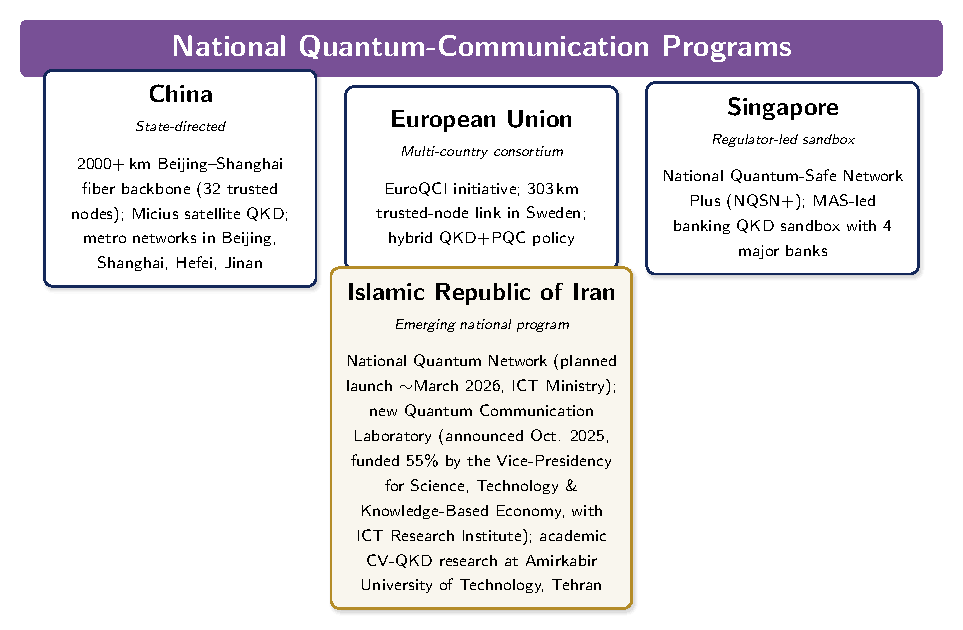
\includegraphics[width=0.98\linewidth]{figs/fig_national_programs.pdf}
% TODO: لوگو، نام‌های پیشنهادی فایل در figs/logos/README.txt
% \vspace{4pt}
% \includegraphics[height=1.1cm]{figs/logos/china.png}\hfill
% \includegraphics[height=1.1cm]{figs/logos/euroqci.png}\hfill
% \includegraphics[height=1.1cm]{figs/logos/singapore.png}\hfill
% \includegraphics[height=1.1cm]{figs/logos/iran.png}
\caption{مقایسهٔ برنامه‌های ملی ارتباطات کوانتومی، شامل جایگاه نوظهور جمهوری اسلامی ایران \Cite{tehrantimes2025network,tqi2025iranlab,iqt2021iranqkd,arxiv2506cvqkd_iran}}
\label{fig:national}
\end{figure}

\textbf{نتیجه‌گیری برای این پروپوزال:} وجود این زیرساخت اولیهٔ سیاستی، آزمایشگاهی و آکادمیک به این معناست که طرح پیشنهادی فصل \ref{chap:tehran} یک آغاز از صفر نیست، بلکه می‌تواند مستقیماً با برنامهٔ ملی شبکهٔ کوانتومی (بند اول بالا) و آزمایشگاه تازه‌تأسیس ارتباطات کوانتومی هم‌راستا و مکمل شود، به‌ویژه با تمرکز اختصاصی این سند بر \textbf{کاربرد بانکی} که در گزارش‌های عمومی موجود دربارهٔ برنامهٔ ملی، هنوز به‌صراحت هدف‌گذاری نشده است.

\section{جمع‌بندی تطبیقی}

جدول \ref{tab:countries} خلاصه‌ای تطبیقی از رویکرد کشورهای مختلف را ارائه می‌دهد.

\begin{table}[htbp]
\centering
\caption{مقایسهٔ تجربهٔ بین‌المللی پیاده‌سازی \lr{QKD}}
\label{tab:countries}
\small
\begin{tabular}{p{2.2cm}p{3.6cm}p{3.6cm}p{4.2cm}}
\toprule
\textbf{کشور/منطقه} & \textbf{مقیاس اصلی} & \textbf{رویکرد راهبردی} & \textbf{کاربرد برجسته} \\
\midrule
چین & ملی/بین‌شهری ($2000$+ کیلومتر) & دولت‌محور، یکپارچه با استانداردسازی بین‌المللی & دولتی، مالی، ماهواره‌ای \\
اروپا (\lr{EuroQCI}) & ملی/منطقه‌ای & کنسرسیوم چندکشوره؛ تمرکز بر \lr{PQC} به‌همراه \lr{QKD} & زیرساخت حیاتی \\
سنگاپور & کلان‌شهری/ملی کوچک & همکاری دولت-بانک-فناور در قالب \lr{Sandbox} & بانکداری \\
ایران (نوظهور) & ملی (در حال طراحی) & دولت‌محور با مشارکت دانشگاهی؛ در آغاز راه & پژوهشی/زیرساختی \\
آمریکا & سازمانی/شرکتی & بخش خصوصی پیشرو (بانک‌ها)؛ سیاست رسمی متمایل به \lr{PQC} & مالی، بلاک‌چین \\
\bottomrule
\end{tabular}
\end{table}

%=====================================================================
